\documentclass[xetex,mathserif,serif,10pt]{beamer}
%\documentclass[11pt]{article}
\usepackage{xltxtra}
\usepackage{polyglossia}
\setdefaultlanguage[spelling=modern]{russian}
%\setmainfont[Mapping=tex-text]{DejaVu Sans}
%\setmainfont[Mapping=tex-text]{Liberation Sans}
\setmonofont[Mapping=tex-text]{DejaVu Sans Mono}
\setmainfont[Mapping=tex-text]{Linux Libertine O}
%\setmonofont[Mapping=tex-text]{Liberation Mono}

\input dot2tex

\usepackage{verbatim}
\usepackage{tabularx}
\usepackage{float}
\usepackage{url}

\usepackage{textpos}

\usepackage{hyperref}

\usepackage{indentfirst}

\usepackage{algorithm}
\usepackage{algorithmic}

\usepackage{graphicx}

\usepackage{listings}
\lstset{ %
language=C++,                   % the language of the code
basicstyle=\ttfamily\footnotesize,% the size of the fonts that are used for the code
numbers=left,                   % where to put the line-numbers
numberstyle=\footnotesize,      % the size of the fonts that are used for the line-numbers
stepnumber=2,                   % the step between two line-numbers. If it's 1, each line
                                % will be numbered
numbersep=5pt,                  % how far the line-numbers are from the code
%backgroundcolor=\color{white},  % choose the background color. You must add \usepackage{color}
showspaces=false,               % show spaces adding particular underscores
showstringspaces=false,         % underline spaces within strings
showtabs=false,                 % show tabs within strings adding particular underscores
frame=single,                   % adds a frame around the code
tabsize=2,                      % sets default tabsize to 2 spaces
captionpos=b,                   % sets the caption-position to bottom
breaklines=true,                % sets automatic line breaking
breakatwhitespace=false,        % sets if automatic breaks should only happen at whitespace
%title=\lstname,                 % show the filename of files included with \lstinputlisting;
                                % also try caption instead of title
escapeinside={\%*}{*)},         % if you want to add a comment within your code
morekeywords={*,...}            % if you want to add more keywords to the set
}

%\setbeamertemplate{caption}[numbered]
\setbeamertemplate{footline}[frame number]

\input config

%\usetheme{Warsaw}
\usetheme{Singapore}

\newenvironment{sframe}[2]{\section{#1}\begin{frame}[label=#2]{#1}}{\end{frame}}

\begin{document}
    \title[BACS]{BACS ACM Contest System}
    \author[Филиппов]{А.~Филиппов\inst{1}}
    \institute
    {
        \inst{1}
        Ижевский государственный технический университет имени М.Т.~Калашникова
    }
    %\frame{\titlepage}

    \input beamertitle.tex

    \begin{sframe}{Цель работы}{target}
        \begin{block}{Цель}
            Разработать тестирующую систему как основу для разработки
            автоматизированных систем проведения соревнований по программированию
        \end{block}

        \begin{block}{Требования}
            \begin{itemize}
                \item API -- программный интерфейс
                \item Расширяемость
                \item Модульность
            \end{itemize}
        \end{block}
    \end{sframe}

    \begin{sframe}{Задачи работы}{problems}
        \begin{itemize}
            \item \hyperlink{systemdesign}{Проектирование тестирующей системы}
            \item \hyperlink{dcs}{Разработка системы распределения нагрузки}
            \item \hyperlink{bunsanpm}{Разработка пакетного менеджера}
            \item \hyperlink{bacsarchive}{Разработка архива задач}
            \item \hyperlink{bacsproblem}{Разработка форматов задач}
            \item \hyperlink{bacsstatementprovider}{Разработка сервиса условий}
        \end{itemize}
    \end{sframe}

    \begin{sframe}{Архитектура системы}{systemdesign}
        \begin{block}{}
            \begin{figure}[H]
                \centering
                \includegraphics{rs/systemdesign}
            \end{figure}
        \end{block}
    \end{sframe}

    \begin{sframe}{Система распределения нагрузки}{dcs}
        \begin{figure}
            \centering
            \includegraphics[width=\columnwidth]{rs/bunsandcs}
        \end{figure}
    \end{sframe}

    \begin{frame}{Система распределения нагрузки: интеграция}
        \begin{figure}
            \centering
            \includegraphics[width=\columnwidth]{rs/bunsandcsbacs}
        \end{figure}
    \end{frame}
    
    \begin{frame}{Система распределения нагрузки: пример работы}
        \begin{itemize}
            \item Сервис регистрируется
            \item Клиент получает URI сервиса по известному идентификатору
            \item Клиент обращается к сервису
        \end{itemize}
        \begin{figure}
            \centering
            \includegraphics[width=\columnwidth]{rs/bunsandcsexample}
        \end{figure}
    \end{frame}

    \begin{sframe}{Пакетный менеджер}{bunsanpm}
        \begin{itemize}
            \item Удалённый репозиторий
            \item Кэширование промежуточных результатов
            \item Компиляция на целевой машине
        \end{itemize}
        \begin{figure}
            \centering
            \includegraphics[width=0.8\columnwidth]{rs/bunsanpm}
        \end{figure}
    \end{sframe}

    \begin{sframe}{Архив задач}{bacsarchive}
        \begin{itemize}
            \item Пользователь добавляет задачу в архив в одном из поддерживаемых форматов.
            \item Архив преобразует задачу из пользовательского формата во внутренний --
                множество пакетов, которые помещаются в репозиторий.
            \item Пользователю предоставляется доступ к информации о задаче
                (название, авторы, отвественные, рекомендуемые настройки проверки, ...).
        \end{itemize}
        \begin{figure}
            \centering
            \includegraphics[width=0.6\columnwidth]{rs/bacsarchive}
        \end{figure}
    \end{sframe}

    \begin{sframe}{Форматы задач}{bacsproblem}
        \begin{itemize}
            \item Поддержка пользовательских форматов задач
            \item Лёгкость добавления поддержки новых форматов
            \item Преобразование в универсальный внутренний формат
        \end{itemize}
    \end{sframe}

    \begin{sframe}{Сервис условий}{bacsstatementprovider}
        \begin{itemize}
            \item Пользователь запрашивает условие у WEB-интерфейса
            \item WEB-интерфейс переадресует запрос сервису условий
            \item Сервис условий генерирует условие из исходного кода,
                находящегося в репозитории
            \item Сервис условий предоставляет пользователю доступ к условию
        \end{itemize}
        \begin{figure}
            \centering
            \includegraphics[width=\columnwidth]{rs/bacsstatementprovider}
        \end{figure}
    \end{sframe}

    \begin{sframe}{Пример работы системы тестирования}{testing}
        \begin{figure}
            \centering
            \includegraphics[width=\columnwidth]{rs/testing}
        \end{figure}
    \end{sframe}

    \begin{frame}{Отправка решения участником}
        \begin{figure}
            \centering
            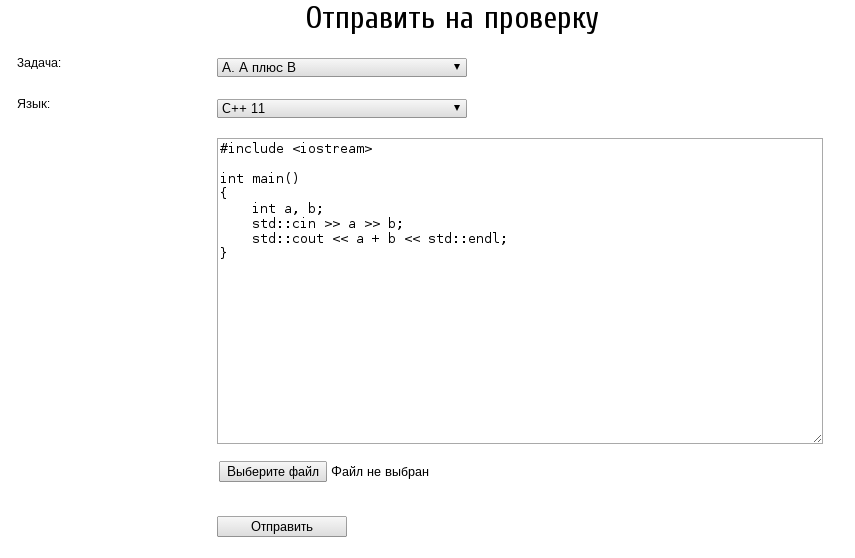
\includegraphics[width=\columnwidth]{rs/sendsubmitok}
        \end{figure}
    \end{frame}
    
    \begin{frame}{Формируемый запрос: системные параметры}
        \lstinputlisting{rs/task_system.txt}
    \end{frame}

    \begin{frame}{Формируемый запрос: решение}
        \lstinputlisting{rs/task_solution.txt}
    \end{frame}

    \begin{frame}{Формируемый запрос: настройки тестирования}
        \lstinputlisting{rs/task_testing.txt}
    \end{frame}

    \begin{frame}{Формируемый запрос: создание файлов}
        \lstinputlisting{rs/task_testing_files.txt}
    \end{frame}

    \begin{frame}{Формируемый запрос: перенаправление ввода-вывода}
        \lstinputlisting{rs/task_testing_execution.txt}
    \end{frame}

    \begin{frame}{Отображение результатов пользователю}
        \begin{figure}
            \centering
            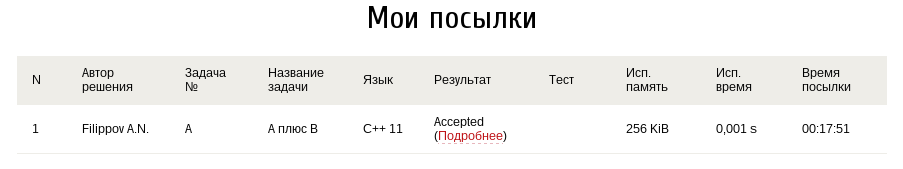
\includegraphics[width=\columnwidth]{rs/mysubmitsok}
        \end{figure}
    \end{frame}

    \begin{frame}
        \Large\centering Спасибо за внимание!
    \end{frame}

    \begin{frame}{Содержание}
        \tableofcontents
    \end{frame}
\end{document}
